\documentclass[twoside]{book}

% Packages required by doxygen
\usepackage{fixltx2e}
\usepackage{calc}
\usepackage{doxygen}
\usepackage[export]{adjustbox} % also loads graphicx
\usepackage{graphicx}
\usepackage[utf8]{inputenc}
\usepackage{makeidx}
\usepackage{multicol}
\usepackage{multirow}
\PassOptionsToPackage{warn}{textcomp}
\usepackage{textcomp}
\usepackage[nointegrals]{wasysym}
\usepackage[table]{xcolor}

% Font selection
\usepackage[T1]{fontenc}
\usepackage[scaled=.90]{helvet}
\usepackage{courier}
\usepackage{amssymb}
\usepackage{sectsty}
\renewcommand{\familydefault}{\sfdefault}
\allsectionsfont{%
  \fontseries{bc}\selectfont%
  \color{darkgray}%
}
\renewcommand{\DoxyLabelFont}{%
  \fontseries{bc}\selectfont%
  \color{darkgray}%
}
\newcommand{\+}{\discretionary{\mbox{\scriptsize$\hookleftarrow$}}{}{}}

% Page & text layout
\usepackage{geometry}
\geometry{%
  a4paper,%
  top=2.5cm,%
  bottom=2.5cm,%
  left=2.5cm,%
  right=2.5cm%
}
\tolerance=750
\hfuzz=15pt
\hbadness=750
\setlength{\emergencystretch}{15pt}
\setlength{\parindent}{0cm}
\setlength{\parskip}{0.2cm}
\makeatletter
\renewcommand{\paragraph}{%
  \@startsection{paragraph}{4}{0ex}{-1.0ex}{1.0ex}{%
    \normalfont\normalsize\bfseries\SS@parafont%
  }%
}
\renewcommand{\subparagraph}{%
  \@startsection{subparagraph}{5}{0ex}{-1.0ex}{1.0ex}{%
    \normalfont\normalsize\bfseries\SS@subparafont%
  }%
}
\makeatother

% Headers & footers
\usepackage{fancyhdr}
\pagestyle{fancyplain}
\fancyhead[LE]{\fancyplain{}{\bfseries\thepage}}
\fancyhead[CE]{\fancyplain{}{}}
\fancyhead[RE]{\fancyplain{}{\bfseries\leftmark}}
\fancyhead[LO]{\fancyplain{}{\bfseries\rightmark}}
\fancyhead[CO]{\fancyplain{}{}}
\fancyhead[RO]{\fancyplain{}{\bfseries\thepage}}
\fancyfoot[LE]{\fancyplain{}{}}
\fancyfoot[CE]{\fancyplain{}{}}
\fancyfoot[RE]{\fancyplain{}{\bfseries\scriptsize Generated on Tue Apr 7 2015 11\+:10\+:18 for My Project by Doxygen }}
\fancyfoot[LO]{\fancyplain{}{\bfseries\scriptsize Generated on Tue Apr 7 2015 11\+:10\+:18 for My Project by Doxygen }}
\fancyfoot[CO]{\fancyplain{}{}}
\fancyfoot[RO]{\fancyplain{}{}}
\renewcommand{\footrulewidth}{0.4pt}
\renewcommand{\chaptermark}[1]{%
  \markboth{#1}{}%
}
\renewcommand{\sectionmark}[1]{%
  \markright{\thesection\ #1}%
}

% Indices & bibliography
\usepackage{natbib}
\usepackage[titles]{tocloft}
\setcounter{tocdepth}{3}
\setcounter{secnumdepth}{5}
\makeindex

% Hyperlinks (required, but should be loaded last)
\usepackage{ifpdf}
\ifpdf
  \usepackage[pdftex,pagebackref=true]{hyperref}
\else
  \usepackage[ps2pdf,pagebackref=true]{hyperref}
\fi
\hypersetup{%
  colorlinks=true,%
  linkcolor=blue,%
  citecolor=blue,%
  unicode%
}

% Custom commands
\newcommand{\clearemptydoublepage}{%
  \newpage{\pagestyle{empty}\cleardoublepage}%
}


%===== C O N T E N T S =====

\begin{document}

% Titlepage & ToC
\hypersetup{pageanchor=false,
             bookmarks=true,
             bookmarksnumbered=true,
             pdfencoding=unicode
            }
\pagenumbering{roman}
\begin{titlepage}
\vspace*{7cm}
\begin{center}%
{\Large My Project }\\
\vspace*{1cm}
{\large Generated by Doxygen 1.8.9.1}\\
\vspace*{0.5cm}
{\small Tue Apr 7 2015 11:10:18}\\
\end{center}
\end{titlepage}
\clearemptydoublepage
\tableofcontents
\clearemptydoublepage
\pagenumbering{arabic}
\hypersetup{pageanchor=true}

%--- Begin generated contents ---
\chapter{Hierarchical Index}
\section{Class Hierarchy}
This inheritance list is sorted roughly, but not completely, alphabetically\+:\begin{DoxyCompactList}
\item \contentsline{section}{Collision}{\pageref{class_collision}}{}
\item \contentsline{section}{Game\+Object}{\pageref{class_game_object}}{}
\begin{DoxyCompactList}
\item \contentsline{section}{Cannon}{\pageref{class_cannon}}{}
\item \contentsline{section}{Flying\+Object}{\pageref{class_flying_object}}{}
\end{DoxyCompactList}
\item \contentsline{section}{Text}{\pageref{class_text}}{}
\item \contentsline{section}{Util}{\pageref{class_util}}{}
\end{DoxyCompactList}

\chapter{Class Index}
\section{Class List}
Here are the classes, structs, unions and interfaces with brief descriptions\+:\begin{DoxyCompactList}
\item\contentsline{section}{\hyperlink{class_cannon}{Cannon} }{\pageref{class_cannon}}{}
\item\contentsline{section}{\hyperlink{class_collision}{Collision} }{\pageref{class_collision}}{}
\item\contentsline{section}{\hyperlink{class_flying_object}{Flying\+Object} }{\pageref{class_flying_object}}{}
\item\contentsline{section}{\hyperlink{class_game_object}{Game\+Object} }{\pageref{class_game_object}}{}
\item\contentsline{section}{\hyperlink{class_text}{Text} }{\pageref{class_text}}{}
\item\contentsline{section}{\hyperlink{class_util}{Util} }{\pageref{class_util}}{}
\end{DoxyCompactList}

\chapter{Class Documentation}
\hypertarget{class_cannon}{}\section{Cannon Class Reference}
\label{class_cannon}\index{Cannon@{Cannon}}
Inheritance diagram for Cannon\+:\begin{figure}[H]
\begin{center}
\leavevmode
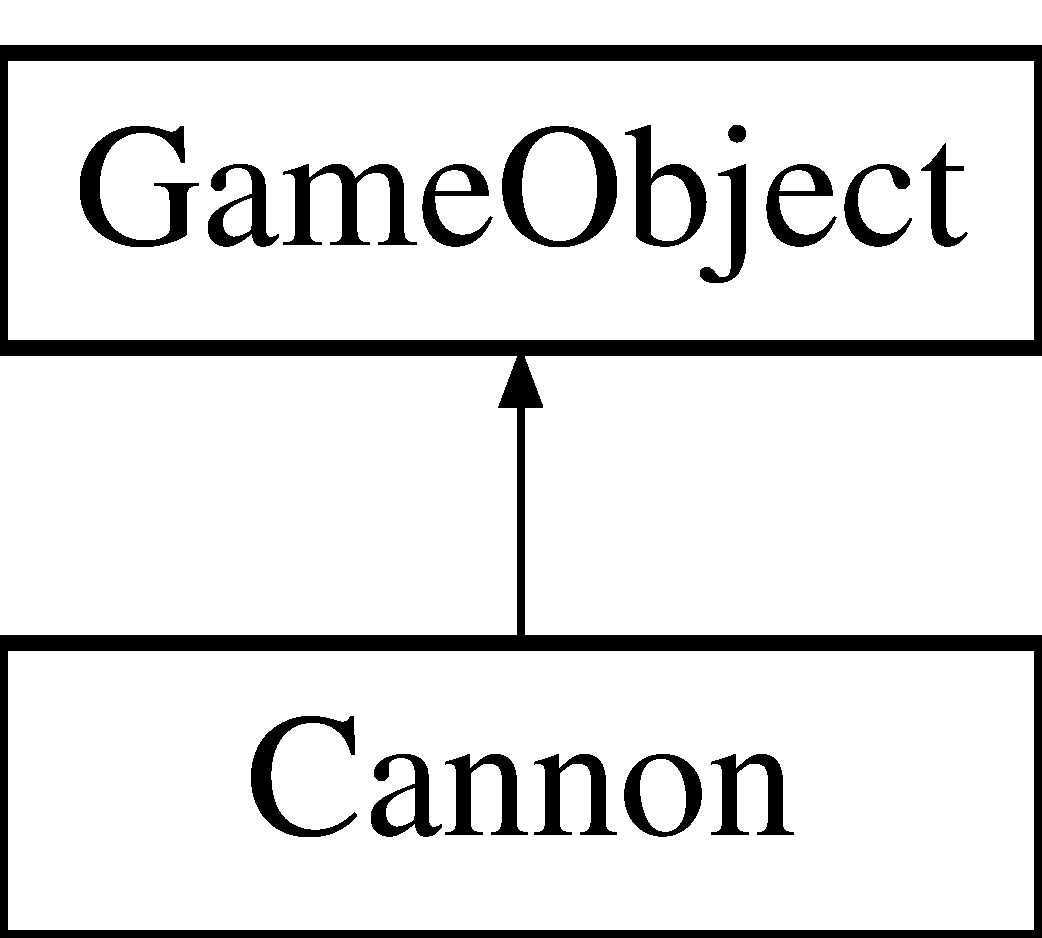
\includegraphics[height=2.000000cm]{class_cannon}
\end{center}
\end{figure}
\subsection*{Public Member Functions}
\begin{DoxyCompactItemize}
\item 
\hypertarget{class_cannon_a235ec1b7acb03815befa09782d5e8055}{}{\bfseries Cannon} (int x, int y, int w, int h, double vel)\label{class_cannon_a235ec1b7acb03815befa09782d5e8055}

\item 
\hypertarget{class_cannon_a8cd5846a20ccd9ec1ce0a732e1de6732}{}{\bfseries Cannon} (int x, int y, int w, int h, double vel, std\+::string path, S\+D\+L\+\_\+\+Renderer $\ast$rend, std\+::string path\+Bullet)\label{class_cannon_a8cd5846a20ccd9ec1ce0a732e1de6732}

\item 
\hypertarget{class_cannon_a7f79c0b940ac84f9f64aa06edece297f}{}void {\bfseries draw} (S\+D\+L\+\_\+\+Renderer $\ast$g\+Renderer) override\label{class_cannon_a7f79c0b940ac84f9f64aa06edece297f}

\item 
\hypertarget{class_cannon_a9363f44cb46f40fe20dcafc51b480be8}{}S\+D\+L\+\_\+\+Texture $\ast$ {\bfseries get\+Texture} (S\+D\+L\+\_\+\+Renderer $\ast$rend, std\+::string path)\label{class_cannon_a9363f44cb46f40fe20dcafc51b480be8}

\item 
\hypertarget{class_cannon_a88acc51fd9109422198053ebe97141df}{}void {\bfseries fire} ()\label{class_cannon_a88acc51fd9109422198053ebe97141df}

\end{DoxyCompactItemize}
\subsection*{Public Attributes}
\begin{DoxyCompactItemize}
\item 
\hypertarget{class_cannon_ae0d033a24c622ee1e9c7ab9888552040}{}std\+::vector$<$ \hyperlink{class_game_object}{Game\+Object} $>$ {\bfseries bullets}\label{class_cannon_ae0d033a24c622ee1e9c7ab9888552040}

\item 
\hypertarget{class_cannon_a39e3cd31451ff3d1a9a1b00fad4f5f30}{}S\+D\+L\+\_\+\+Texture $\ast$ {\bfseries bullet\+Texture}\label{class_cannon_a39e3cd31451ff3d1a9a1b00fad4f5f30}

\end{DoxyCompactItemize}


The documentation for this class was generated from the following file\+:\begin{DoxyCompactItemize}
\item 
Cannon.\+h\end{DoxyCompactItemize}

\hypertarget{class_collision}{}\section{Collision Class Reference}
\label{class_collision}\index{Collision@{Collision}}
\subsection*{Static Public Member Functions}
\begin{DoxyCompactItemize}
\item 
\hypertarget{class_collision_ab72868eae1e48ea5c355c109d8cfc912}{}static bool {\bfseries A\+A\+B\+B\+Collision} (S\+D\+L\+\_\+\+Rect $\ast$a, S\+D\+L\+\_\+\+Rect $\ast$b)\label{class_collision_ab72868eae1e48ea5c355c109d8cfc912}

\item 
\hypertarget{class_collision_ac8dc877b6d5d90acd93ff8ad4632fd20}{}static bool {\bfseries Circle\+Collision} (S\+D\+L\+\_\+\+Rect c1, S\+D\+L\+\_\+\+Rect c2)\label{class_collision_ac8dc877b6d5d90acd93ff8ad4632fd20}

\end{DoxyCompactItemize}


The documentation for this class was generated from the following files\+:\begin{DoxyCompactItemize}
\item 
Collision.\+h\item 
Collision.\+cpp\end{DoxyCompactItemize}

\hypertarget{class_flying_object}{}\section{Flying\+Object Class Reference}
\label{class_flying_object}\index{Flying\+Object@{Flying\+Object}}
Inheritance diagram for Flying\+Object\+:\begin{figure}[H]
\begin{center}
\leavevmode
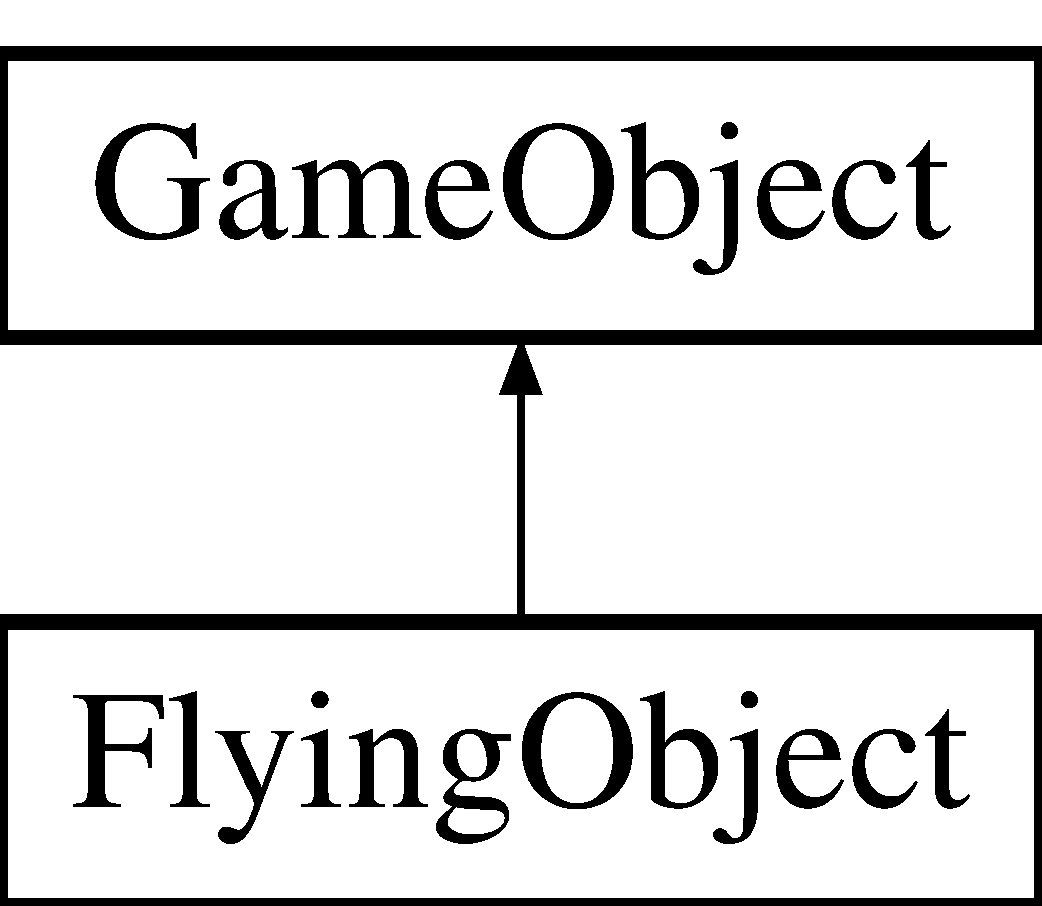
\includegraphics[height=2.000000cm]{class_flying_object}
\end{center}
\end{figure}
\subsection*{Public Member Functions}
\begin{DoxyCompactItemize}
\item 
\hypertarget{class_flying_object_a75bf7eef115a12fcc440406220078f3e}{}bool {\bfseries is\+Is\+Falling} () const \label{class_flying_object_a75bf7eef115a12fcc440406220078f3e}

\item 
\hypertarget{class_flying_object_a7a85cdbe612ff033814800a9a3611113}{}void {\bfseries set\+Is\+Falling} (bool is\+Falling)\label{class_flying_object_a7a85cdbe612ff033814800a9a3611113}

\item 
\hypertarget{class_flying_object_ac3aa6af7e597804ca5e3bb1f23ef7bce}{}{\bfseries Flying\+Object} (int x, int y, int w, int h, double vel)\label{class_flying_object_ac3aa6af7e597804ca5e3bb1f23ef7bce}

\item 
\hypertarget{class_flying_object_ae19d46468cfc5223a67404e5ef2899c9}{}{\bfseries Flying\+Object} (int x, int y, int w, int h, double vel, std\+::string path, S\+D\+L\+\_\+\+Renderer $\ast$rend, std\+::string path\+Bullet)\label{class_flying_object_ae19d46468cfc5223a67404e5ef2899c9}

\item 
\hypertarget{class_flying_object_a24ea9f0837fd8d18bbc51bc435ed86c2}{}void {\bfseries draw} (S\+D\+L\+\_\+\+Renderer $\ast$g\+Renderer) override\label{class_flying_object_a24ea9f0837fd8d18bbc51bc435ed86c2}

\item 
\hypertarget{class_flying_object_af58bd62f02039544dfd04c3ef854fb33}{}void {\bfseries draw} () override\label{class_flying_object_af58bd62f02039544dfd04c3ef854fb33}

\item 
\hypertarget{class_flying_object_a0a7125dda78155f497259007ea219314}{}S\+D\+L\+\_\+\+Texture $\ast$ {\bfseries get\+Texture} (S\+D\+L\+\_\+\+Renderer $\ast$rend, std\+::string path)\label{class_flying_object_a0a7125dda78155f497259007ea219314}

\item 
\hypertarget{class_flying_object_a9bc37c29f698d99102173560612f882d}{}void {\bfseries fire} ()\label{class_flying_object_a9bc37c29f698d99102173560612f882d}

\item 
\hypertarget{class_flying_object_a9b75bff7e78524dbb39d398f1f3a8702}{}void {\bfseries set\+Texture\+Body} (S\+D\+L\+\_\+\+Texture $\ast$t)\label{class_flying_object_a9b75bff7e78524dbb39d398f1f3a8702}

\item 
\hypertarget{class_flying_object_a7fe6ad261feebe138e7b0aa505cde139}{}void {\bfseries set\+Texture\+Bullet} (S\+D\+L\+\_\+\+Texture $\ast$t)\label{class_flying_object_a7fe6ad261feebe138e7b0aa505cde139}

\item 
\hypertarget{class_flying_object_ad6df1d7fc43370822a889519328b2e58}{}void {\bfseries stop\+Falling} ()\label{class_flying_object_ad6df1d7fc43370822a889519328b2e58}

\item 
\hypertarget{class_flying_object_aaccd1a04a85a36e0481234a9800cae9f}{}void {\bfseries fall} ()\label{class_flying_object_aaccd1a04a85a36e0481234a9800cae9f}

\item 
\hypertarget{class_flying_object_ad5df5f8b0caed1b1437e033b9c83dd6e}{}void {\bfseries update\+Speed\+X} (double acceleration, double d\+Time)\label{class_flying_object_ad5df5f8b0caed1b1437e033b9c83dd6e}

\item 
\hypertarget{class_flying_object_a8ce65d5d92854d92d456f050b8187d0a}{}void {\bfseries update\+Speed\+Y} (double acceleration, double d\+Time)\label{class_flying_object_a8ce65d5d92854d92d456f050b8187d0a}

\end{DoxyCompactItemize}
\subsection*{Public Attributes}
\begin{DoxyCompactItemize}
\item 
\hypertarget{class_flying_object_a350b186c309d32d0de570c7a2d57ac81}{}std\+::vector$<$ \hyperlink{class_game_object}{Game\+Object} $>$ {\bfseries bullets}\label{class_flying_object_a350b186c309d32d0de570c7a2d57ac81}

\item 
\hypertarget{class_flying_object_a321b6cbde4049c3b92025b91d6d55353}{}S\+D\+L\+\_\+\+Texture $\ast$ {\bfseries bullet\+Texture}\label{class_flying_object_a321b6cbde4049c3b92025b91d6d55353}

\end{DoxyCompactItemize}


The documentation for this class was generated from the following file\+:\begin{DoxyCompactItemize}
\item 
Flying\+Object.\+h\end{DoxyCompactItemize}

\hypertarget{class_game_object}{}\section{Game\+Object Class Reference}
\label{class_game_object}\index{Game\+Object@{Game\+Object}}
Inheritance diagram for Game\+Object\+:\begin{figure}[H]
\begin{center}
\leavevmode
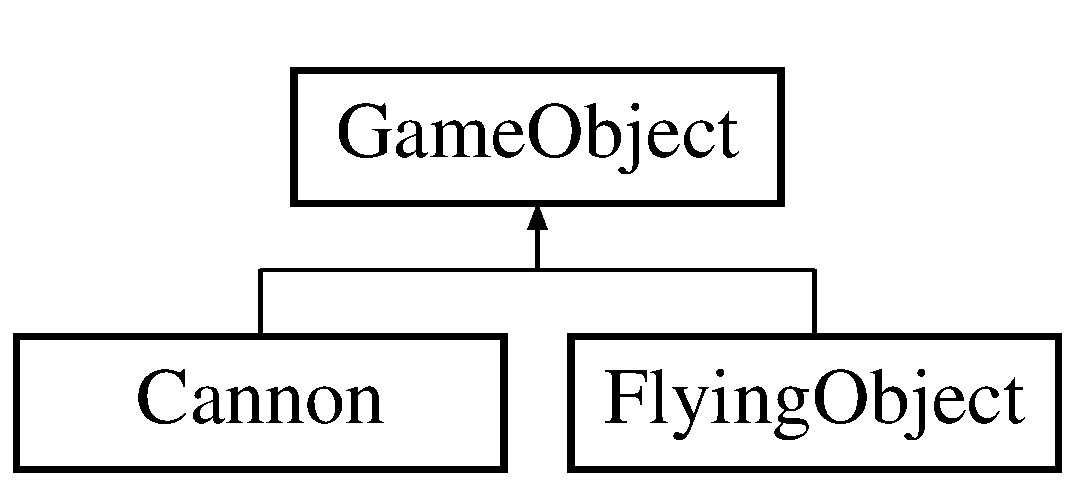
\includegraphics[height=2.000000cm]{class_game_object}
\end{center}
\end{figure}
\subsection*{Public Member Functions}
\begin{DoxyCompactItemize}
\item 
\hypertarget{class_game_object_ad5223d5e6c6bc39529c85dceb1d50930}{}{\bfseries Game\+Object} (int x, int y, int w, int h)\label{class_game_object_ad5223d5e6c6bc39529c85dceb1d50930}

\item 
\hypertarget{class_game_object_a3a91505bf2480eab8333df4c9c6b5a7e}{}{\bfseries Game\+Object} (int x, int y, int w, int h, double speed)\label{class_game_object_a3a91505bf2480eab8333df4c9c6b5a7e}

\item 
\hypertarget{class_game_object_a36a5f15c226732b4ecea0cd01d6c0c37}{}{\bfseries Game\+Object} (int x, int y, int w, int h, double vel, std\+::string path, S\+D\+L\+\_\+\+Renderer $\ast$rend)\label{class_game_object_a36a5f15c226732b4ecea0cd01d6c0c37}

\item 
\hypertarget{class_game_object_a508ffb146e68ae0699c16e7e0be395cf}{}void {\bfseries move\+X} (double d\+Time)\label{class_game_object_a508ffb146e68ae0699c16e7e0be395cf}

\item 
\hypertarget{class_game_object_a8c98efc0e75c4df16d6d065dbf119f4a}{}void {\bfseries move\+Y} (double d\+Time)\label{class_game_object_a8c98efc0e75c4df16d6d065dbf119f4a}

\item 
\hypertarget{class_game_object_a29a1e18b85acfbdccca5388b6b11d6e6}{}void {\bfseries set\+Speed\+X} (double v)\label{class_game_object_a29a1e18b85acfbdccca5388b6b11d6e6}

\item 
\hypertarget{class_game_object_a11263a87aad0ff22157eaf48d9e603e3}{}void {\bfseries set\+Speed\+Y} (double v)\label{class_game_object_a11263a87aad0ff22157eaf48d9e603e3}

\item 
\hypertarget{class_game_object_ac3c1034c2b4645b10a57198516f0c66e}{}void {\bfseries update\+Speed\+X} (double acceleration, double d\+Time)\label{class_game_object_ac3c1034c2b4645b10a57198516f0c66e}

\item 
\hypertarget{class_game_object_a76a96005333af8f0b2d7c6dbe1ecbeaf}{}void {\bfseries update\+Speed\+Y} (double acceleration, double d\+Time)\label{class_game_object_a76a96005333af8f0b2d7c6dbe1ecbeaf}

\item 
\hypertarget{class_game_object_a0872c027418d59fa7cb3385c0157331c}{}void {\bfseries set\+Texture} (S\+D\+L\+\_\+\+Texture $\ast$tex)\label{class_game_object_a0872c027418d59fa7cb3385c0157331c}

\item 
\hypertarget{class_game_object_a149810a726d5f0f0928e3cc1e2f35caa}{}virtual void {\bfseries draw} (S\+D\+L\+\_\+\+Renderer $\ast$g\+Renderer)\label{class_game_object_a149810a726d5f0f0928e3cc1e2f35caa}

\item 
\hypertarget{class_game_object_abb64143e72358beb808db22182517802}{}virtual void {\bfseries draw} ()\label{class_game_object_abb64143e72358beb808db22182517802}

\item 
\hypertarget{class_game_object_a1bd14aa169f501f94f1721943d716535}{}void {\bfseries Update} ()\label{class_game_object_a1bd14aa169f501f94f1721943d716535}

\item 
\hypertarget{class_game_object_a02f615d4d777a5542f7bcb757462d212}{}S\+D\+L\+\_\+\+Texture $\ast$ {\bfseries get\+Texture} (std\+::string path)\label{class_game_object_a02f615d4d777a5542f7bcb757462d212}

\item 
\hypertarget{class_game_object_ae726f13a135d68908628299d702c88f4}{}void {\bfseries fall} ()\label{class_game_object_ae726f13a135d68908628299d702c88f4}

\item 
\hypertarget{class_game_object_a759f927dbbb6e388acb332bbe76ded59}{}void {\bfseries stop\+Falling} ()\label{class_game_object_a759f927dbbb6e388acb332bbe76ded59}

\end{DoxyCompactItemize}
\subsection*{Public Attributes}
\begin{DoxyCompactItemize}
\item 
\hypertarget{class_game_object_a01accf16dabf8b1006e3df597dc1728a}{}S\+D\+L\+\_\+\+Texture $\ast$ {\bfseries texture}\label{class_game_object_a01accf16dabf8b1006e3df597dc1728a}

\item 
\hypertarget{class_game_object_af6009d73be98a4bd54272d06b50f2eac}{}S\+D\+L\+\_\+\+Rect {\bfseries position}\label{class_game_object_af6009d73be98a4bd54272d06b50f2eac}

\item 
\hypertarget{class_game_object_aca8078da92a2d34889e428708d501246}{}S\+D\+L\+\_\+\+Renderer $\ast$ {\bfseries obj\+Rend}\label{class_game_object_aca8078da92a2d34889e428708d501246}

\item 
\hypertarget{class_game_object_a71fe4978f8508ada95019f5fc77fd8c6}{}double {\bfseries speed\+X}\label{class_game_object_a71fe4978f8508ada95019f5fc77fd8c6}

\item 
\hypertarget{class_game_object_a09a14839f77f2eded95fbf82204e1f1c}{}double {\bfseries speed\+Y}\label{class_game_object_a09a14839f77f2eded95fbf82204e1f1c}

\item 
\hypertarget{class_game_object_a127eb9388ff0cdbbd20f000b24420564}{}uint32\+\_\+t {\bfseries time\+Start}\label{class_game_object_a127eb9388ff0cdbbd20f000b24420564}

\item 
\hypertarget{class_game_object_af52441e1d468ad926cfe265afc6734de}{}uint32\+\_\+t {\bfseries delta\+T}\label{class_game_object_af52441e1d468ad926cfe265afc6734de}

\item 
\hypertarget{class_game_object_a0ee7d3e2f3cfdeba9d924abe12d6739a}{}uint32\+\_\+t {\bfseries current\+Time}\label{class_game_object_a0ee7d3e2f3cfdeba9d924abe12d6739a}

\end{DoxyCompactItemize}


The documentation for this class was generated from the following files\+:\begin{DoxyCompactItemize}
\item 
Game\+Object.\+h\item 
Game\+Object.\+cpp\end{DoxyCompactItemize}

\hypertarget{class_text}{}\section{Text Class Reference}
\label{class_text}\index{Text@{Text}}
\subsection*{Public Attributes}
\begin{DoxyCompactItemize}
\item 
\hypertarget{class_text_a881e261364e0678ddcf6865bf9d668b9}{}S\+D\+L\+\_\+\+Surface $\ast$ {\bfseries surface}\label{class_text_a881e261364e0678ddcf6865bf9d668b9}

\item 
\hypertarget{class_text_abfd7707d427d99386fa552cd4a114487}{}S\+D\+L\+\_\+\+Rect {\bfseries rect}\label{class_text_abfd7707d427d99386fa552cd4a114487}

\item 
\hypertarget{class_text_ae23ac53acb57e760b91c81d8c4aec8c7}{}T\+T\+F\+\_\+\+Font $\ast$ {\bfseries font}\label{class_text_ae23ac53acb57e760b91c81d8c4aec8c7}

\item 
\hypertarget{class_text_ab0f771bd18d8e968f7aaee4a4e26e385}{}S\+D\+L\+\_\+\+Color {\bfseries color}\label{class_text_ab0f771bd18d8e968f7aaee4a4e26e385}

\item 
\hypertarget{class_text_aea2a82ef1d8b4d448b6b3e524bce2cc2}{}S\+D\+L\+\_\+\+Texture $\ast$ {\bfseries texture}\label{class_text_aea2a82ef1d8b4d448b6b3e524bce2cc2}

\item 
\hypertarget{class_text_a1628dc5c1a3c44d1aefa9a329b99ce7d}{}std\+::string {\bfseries display\+Text}\label{class_text_a1628dc5c1a3c44d1aefa9a329b99ce7d}

\end{DoxyCompactItemize}


The documentation for this class was generated from the following files\+:\begin{DoxyCompactItemize}
\item 
Text.\+h\item 
Text.\+cpp\end{DoxyCompactItemize}

\hypertarget{class_util}{}\section{Util Class Reference}
\label{class_util}\index{Util@{Util}}
\subsection*{Static Public Member Functions}
\begin{DoxyCompactItemize}
\item 
\hypertarget{class_util_af9e2112ba400436dd749539bdeffea5b}{}static int {\bfseries Generate\+Random} (int l, int u)\label{class_util_af9e2112ba400436dd749539bdeffea5b}

\end{DoxyCompactItemize}


The documentation for this class was generated from the following files\+:\begin{DoxyCompactItemize}
\item 
Util.\+h\item 
Util.\+cpp\end{DoxyCompactItemize}

%--- End generated contents ---

% Index
\backmatter
\newpage
\phantomsection
\clearemptydoublepage
\addcontentsline{toc}{chapter}{Index}
\printindex

\end{document}
